\documentclass[xcolor=x11names]{beamer}
%%%%%%%%%%%%%%%%%%%%%%%%%%%%%%%%%%%%%%%%%%%%%%%%%%%%%%%%%%%%
%%  This Beamer template was created by Cameron Bracken.
%%  Anyone can freely use or modify it for any purpose
%%  without attribution.
%%
%%  Last Modified by C. Bracken: January 9, 2009
%%
%%  The preamble, and maybe some modification of the Cameron Bracken's template is due to Attila Molnár.
%%
%%

%% General document
\usepackage[utf8]{inputenc}
\usepackage[T1]{fontenc}
\usepackage{graphicx}
\usepackage{tikz}
\usetikzlibrary{decorations.fractals}
\usetikzlibrary{decorations.text}
\usepgflibrary{arrows}
\usetikzlibrary{fadings}
\usetikzlibrary[decorations.pathmorphing]
\tikzfading[name=fade inside, inner color=transparent!70, outer color=transparent!70]
\usetikzlibrary{calc}
\usetikzlibrary{intersections}
\usetikzlibrary{shapes}
\usetikzlibrary{patterns}
\usefonttheme{serif}
\usepackage{amssymb} 			
\usepackage{amsmath}
\usepackage{ifthen}
\usepackage[normalem]{ulem}
\usepackage{mathrsfs}

%%%%%%%%%%%%%%%%%%%%%%%%%%%%%%%%%%%%%%%%%%%%%%%%%%%%%%%%%%%%%%%%%%%%%%%%%%%%%%%%%%%%
%% Beamer Layout %%%%%%%%%%%%%%%%%%%%%%%%%%%%%%%%%%
\useoutertheme[subsection=false,shadow]{miniframes}
\useinnertheme{default}
\usefonttheme{serif}
%\usepackage{txfonts} %Hook for strict implication!
\DeclareSymbolFont{symbolsC}{U}{txsyc}{m}{n}
\DeclareMathSymbol{\strictif}{\mathrel}{symbolsC}{74}
\DeclareMathSymbol{\boxright}{\mathrel}{symbolsC}{128}
\usepackage{palatino}
%\usepackage[uppercase=upright,charter]{mathdesign}

\setbeamerfont{title like}{shape=\scshape}
\setbeamerfont{frametitle}{shape=\scshape}


\setbeamercolor*{lower separation line head}{bg=white!40!DeepSkyBlue3}
\setbeamercolor*{normal text}{fg=black,bg=white}
\setbeamercolor*{alerted text}{fg=red}
\setbeamercolor*{example text}{fg=black}
\setbeamercolor*{structure}{fg=black}

\setbeamercolor*{palette tertiary}{fg=black,bg=white!90!DeepSkyBlue3}
\setbeamercolor*{palette quaternary}{fg=black,bg=black!10}

%\setbeamercolor{block body alerted}{bg=normal text.bg!90!DeepSkyBlue4}
\setbeamercolor{block body}{bg=normal text.bg!95!DeepSkyBlue3}
%\setbeamercolor{block body example}{bg=normal text.bg!90!DeepSkyBlue4}
%\setbeamercolor{block title alerted}{use={normal text,alerted text},fg=alerted text.fg!75!normal text.fg,bg=normal text.bg!90!DeepSkyBlue4}
\setbeamercolor{block title}{bg=normal text.bg!70!DeepSkyBlue3}
%\setbeamercolor{block title example}{use={normal text,example text},fg=example text.fg!75!normal text.fg,bg=normal text.bg!75!DeepSkyBlue4}

\setbeamertemplate{blocks}[rounded][shadow=true]
%\setbeamertemplate{background canvas}[vertical shading][bottom=white,top=structure.fg!25]
%\setbeamertemplate{sidebar canvas left}[horizontal shading][left=white!40!black,right=black]
\setbeamertemplate{itemize items}[circle]
\setbeamercolor*{itemize item}{fg=DeepSkyBlue3}
\setbeamercolor*{itemize subitem}{fg=DeepSkyBlue3}
\setbeamercolor*{itemize subsubitem}{fg=DeepSkyBlue3}
\setbeamertemplate{enumerate items}[circle]
%\setbeamercolor{item projected}{bg=DeepSkyBlue3,fg=black}
\setbeamercolor{item projected}{bg=white,fg=DeepSkyBlue3}
\setbeamercolor*{enumerate item}{fg=DeepSkyBlue3}
\setbeamercolor*{enumerate subitem}{fg=DeepSkyBlue3}
\setbeamercolor*{enumerate subsubitem}{fg=DeepSkyBlue3}

%%%%%%%%%%%%%%%%%%%%%%%%%%%%%%%%%%%%%%%%%%%%%%%%%%


%%%%%%%%%%%%%%%%%%%%%%%%%%%%%%%%%%%%%%%%%%%%%%%%%%%%%%%%%%%%%%%%%%%%%%%%%%%%%%%%%%%%

\newenvironment{defi}[1][]{\begin{block}{\footnotesize \textsc{Definition} \ifthenelse{\equal{#1}{}}{}{\, (#1)}}}{\end{block}}
\newenvironment{prop}[1][]{\begin{block}{\footnotesize \textsc{Proposition} \ifthenelse{\equal{#1}{}}{}{\, (\textsc{#1})}}}{\end{block}}
\newenvironment{lemm}[1][]{\begin{block}{\footnotesize \textsc{Lemma} \ifthenelse{\equal{#1}{}}{}{\, (\textsc{#1})}}}{\end{block}}
\newenvironment{idea}[1][]{\begin{block}{\footnotesize \textsc{Idea} \ifthenelse{\equal{#1}{}}{}{\, (\textsc{#1})}}}{\end{block}}
\newenvironment{rema}[1][]{\begin{block}{\footnotesize \textsc{Remark} \ifthenelse{\equal{#1}{}}{}{\, (\textsc{#1})}}}{\end{block}}
\newenvironment{coro}[1][]{\begin{block}{\footnotesize \textsc{Corollary} \ifthenelse{\equal{#1}{}}{}{\, (\textsc{#1})}}}{\end{block}}
\newenvironment{tete}[1][]{\begin{block}{\footnotesize \textsc{Theorem} \ifthenelse{\equal{#1}{}}{}{\, (\textsc{#1})}}}{\end{block}}
\newenvironment{claim}[1][]{\begin{block}{Claim \ifthenelse{\equal{#1}{}}{}{\, (\textsc{#1})}}}{\end{block}}
%\newenvironment{lemma}[1][]{\begin{block}{Lemma \ifthenelse{\equal{#1}{}}{}{\, (\textsc{#1})}}}{\end{block}}
\newenvironment{question}[1][]{\begin{block}{Question \ifthenelse{\equal{#1}{}}{}{\, (\textsc{#1})}}}{\end{block}}
\newenvironment{rem}[1][]{\begin{block}{Remark \ifthenelse{\equal{#1}{}}{}{\, (\textsc{#1})}}}{\end{block}}
\newenvironment{homework}[1][]{\begin{block}{Homework \ifthenelse{\equal{#1}{}}{}{\, (\textsc{#1})}}}{\end{block}}
\newenvironment{proo}[1][]{\begin{block}{\footnotesize \textsc{Proof} \ifthenelse{\equal{#1}{}}{}{\, (\textsc{#1})}}}{\end{block}}

%%%%%%%%%%%%%%%%%%%%%
%% To evade unnecessary circles, mainly for \cimdia
%%%%%%%%%%%%%%%%%%%%%

\makeatletter
\let\beamer@writeslidentry@miniframeson=\beamer@writeslidentry
\def\beamer@writeslidentry@miniframesoff{%
  \expandafter\beamer@ifempty\expandafter{\beamer@framestartpage}{}% does not happen normally
  {%else
    % removed \addtocontents commands
    \clearpage\beamer@notesactions%
  }
}
\newcommand*{\miniframeson}{\let\beamer@writeslidentry=\beamer@writeslidentry@miniframeson}
\newcommand*{\miniframesoff}{\let\beamer@writeslidentry=\beamer@writeslidentry@miniframesoff}
\makeatother

%%%%%%%%%%%%%%%%%%%%%%%%%%%%%
%%%%%%%%%%%%% END %%%%%%%%%%%
%%%%%%%%%%%%%%%%%%%%%%%%%%%%%


%%%% Formatting Commands

\newcommand{\cimdia}[1] {\miniframesoff \begin{frame}\begin{center}\huge \begin{tabular}{c}#1\end{tabular}\end{center}\end{frame}\miniframeson}
\newcommand{\szakasz}[2][]{\section{#1}\subsection{}\cimdia{#2}}
\newcommand{\bluebullet}{\textcolor{DeepSkyBlue3}{\quad $\bullet$} \,\,}

\newenvironment{frame*}[1][]{\miniframesoff \begin{frame} #1}{\end{frame}\miniframeson}

  % for admissible intersections
  \newcommand{\bigsqcap}{\rotatebox[origin=c]{180}{$\bigsqcup$}}

\newcommand{\felkorvonal}[2]{\draw[rounded corners=0] (180+#1:.25*#2 cm) arc (180+#1:360+#1:.25*#2 cm)--cycle;}
\newcommand{\pecset}[2]{\begin{tikzpicture}[remember picture,overlay]
\node [ draw=red, rectangle, rounded corners=5mm, inner sep=1mm, ultra thick, fill=white, fill opacity=.8, rotate=30, scale=#1, text opacity=0.7] at (current page.center) {#2};\end{tikzpicture}}

\newcommand{\felirat}[7][]{\begin{tikzpicture}[remember picture,overlay]
\node [draw=DeepSkyBlue3, rectangle, rounded corners=#3 mm, inner sep=#2mm, ultra thick, fill=white, fill opacity=.8, scale=#4, text opacity=1,#1]
at ([xshift=#5 cm, yshift=#6 cm]current page.center) {#7};
\end{tikzpicture}}

\newcommand{\underconstruction}[1]{\begin{tikzpicture}[remember picture,overlay]
\node [rectangle, rounded corners=5mm, inner sep=1mm, rotate=30, scale=#1, text opacity=0.4]at (current page.center){\textsc{\textcolor{orange}{\begin{tabular}{c}under \\construction\end{tabular}}}};
\end{tikzpicture}}

\newcommand{\dzsa}[1]{\textsc{\underline{#1}}:}
\newcommand{\axiom}[1]{\bemph{(\mathrm{#1})}}



% Emphasizing:
\definecolor{barna}{rgb}{0.5,0.2,0.1}
\newcommand{\bemph}[1] {{\color{DeepSkyBlue3}{#1}}}
\newcommand{\kemph}[1] {{\color{blue}{#1}}}
\newcommand{\cemph}[1]{\textcolor{red}{#1}}
\newcommand{\zemph}[1] {{\color{Green2}{#1}}}
\newcommand{\yemph}[1] {{\color{Orange1}{#1}}}
%\renewcommand{\emph}[1]{\textbf{#1}}

\newcommand{\FD}{\mathbf F}
\newcommand{\FB}{\mathbf G}
\newcommand{\PD}{\mathbf P}
\newcommand{\PB}{\mathbf H}
\newcommand{\GB}{\mathbf A}
\newcommand{\GD}{\mathbf E}

\newcommand{\FDDot}{\underline{\mathbf F}}
\newcommand{\FBDot}{\underline{\mathbf G}}
\newcommand{\PDDot}{\underline{\mathbf P}}
\newcommand{\PBDot}{\underline{\mathbf H}}

\newcommand{\CFD}{\mathbf F^c}
\newcommand{\CFB}{\mathbf G^c}
\newcommand{\CPD}{\mathbf P^c}
\newcommand{\CPB}{\mathbf H^c}

\newcommand{\CFDDot}{\underline{\mathbf F^c}}
\newcommand{\CFBDot}{\underline{\mathbf G^c}}
\newcommand{\CPDDot}{\underline{\mathbf P^c}}
\newcommand{\CPBDot}{\underline{\mathbf H^c}}

\renewcommand{\Diamond}{\scalebox{.9}{\raisebox{-.4ex}{\rotatebox{45}{$\Box$}}}}

%causal
\newcommand{\past}{\succ}
\newcommand{\pasteq}{\succeq}
\newcommand{\future}{\prec}
\newcommand{\futureeq}{\preceq}
%lightlike
\newcommand{\llpast}{\nwarrow}
\newcommand{\llpasteq}{\underline\nwarrow}
\newcommand{\llfuture}{\nearrow}
\newcommand{\llfutureeq}{\mathop{\underline\nearrow}}
%timelike
\newcommand{\tlpast}{\gg}
\newcommand{\tlpasteq}{\underline \gg}
\newcommand{\tlfuture}{\ll}
\newcommand{\tlfutureeq}{\underline \ll}

\newcommand{\egyuttjar}{\mathop{\uparrow \uparrow}}
\newcommand{\Between}{\mathrm{B}}
\newcommand{\EqDist}{\equiv}
\newcommand{\ISCM}{\uparrow\equiv\uparrow}

 \newcommand{\vonal} [1][.2]{\hspace{#1cm} | \hspace{#1cm}}

 \newcommand{\lrule}[3][c]{\begin{array}{#1} #2  \\  \hline #3 \end{array}}
 \newcommand{\dlrule}[3][c]{\begin{array}{#1} #2  \\  \hline\hline #3 \end{array}}
 \newcommand{\dual}{\delta}

 \newcommand{\mono}{\rightarrowtail}
 \newcommand{\epi}{\twoheadrightarrow}
 \newcommand{\iso}{\rightarrowtail \!\!\!\!\! \rightarrow}

 \newcommand{\defegy}[1][.1]{\hspace{#1cm}\overset{\textup{\tiny def}}{=}\hspace{#1cm}}
 \newcommand{\defpont}[1][.1]{\hspace{#1cm}\overset{\textup{\tiny def}}{:}\hspace{#1cm}}
 \newcommand{\defekv}[1][.1]{\hspace{#1cm}\overset{\textup{\tiny def}}{ \Leftrightarrow }\hspace{#1cm}}
 \newcommand{\lthen}{\rightarrow}
 \newcommand{\liff}{\leftrightarrow}
 \newcommand{\forallin}[2]{(\forall #1 \in #2)}
 \newcommand{\existsin}[2]{(\exists #1 \in #2)}
 \newcommand{\nexistsin}[2]{(\nexists #1 \in #2)}
 \newcommand{\forallp}[1]{(\forall #1)}
 \newcommand{\existsp}[1]{(\exists #1)}

 \newcommand{\points}[1][0]{\hspace{#1ex}\hspace{-.5ex}:\hspace{-.5ex}\hspace{#1ex}}
 \newcommand{\Points}{\mathrm{P}}
 \newcommand{\Pointsf}{\mathrm{p}}
 \newcommand{\Ex}{\mathrm{E}}

\newcommand{\wline}[1]{\mathrm{wline}_{#1}}

\newcommand{\magyi}[1]{\textup{\bemph{\tiny #1}}}
\newcommand{\magyarazat}[2]{\overset{\substack{\textup{#2}\\ \downarrow}}{#1}}
\newcommand{\wintension}[3][]{{[}\hspace{-.46mm}{[} {#3}{]}\hspace{-.46mm}{]}^{\mathfrak{#1}}_{#2}}
\newcommand{\canintension}[2][]{{[}\hspace{-.46mm}{[} {#2}{]}\hspace{-.46mm}{]}_{\mathrm{#1}}}
\newcommand{\intension}[2][]{{[}\hspace{-.46mm}{[} {#2}{]}\hspace{-.46mm}{]}^{\mathfrak{#1}}}

\newcommand{\theory}[2][]{\mathrm{th}_{\mathfrak{#1}}(#2)}

\newcommand{\derives}[1][]{\vdash_{\mathrm{#1}}}


\newcommand{\PBTemplate}[1]{{#1} \overrightarrow {\PB}}
\newcommand{\FBTemplate}[1]{{#1} \overrightarrow {\FB}}
\newcommand{\BoxTemplate}[1]{{#1} \overrightarrow {\Box}}
\newcommand{\PDTemplate}[1]{{#1} \widehat {\PD}}
\newcommand{\FDTemplate}[1]{{#1} \widehat {\FD}}
%\newcommand{\DiamondTemplate}[1]{#1\hspace{-.2ex} \mathop{\Diamond\hspace{-1.35ex} \raisebox{.4ex}{\scalebox{.5}{$\land$}}}\,}

%%%%%%%%%%%%%%%%%%%%%%%%%%%%%%%%%%%%%%%%%%%%%%%%%%%%%%
\newenvironment{tomb}[2][.1]{\arraycolsep=#1cm\begin{array}{#2}}{\end{array}}

\beamertemplatenavigationsymbolsempty


\author{Attila Moln\'ar}
\date{2014. March 21.}
\title{Classical investigations \\ of Pointer logics}
\institute{ELTE}
\begin{document}

\begin{frame}
\centering
\textsc{\Large Classical investigations \\ of Pointer logics}

\bigskip

{ \small Attila Moln\'ar

    \textit{E\"otv\"os Lor\'and University}}

 \begin{figure}
\includegraphics[scale=.3]{elte_cimer.png}
 \end{figure}

	\today
\end{frame}


\szakasz[SPTh]{SPTh: State-Pointer Theory}
\begin{frame}
	\frametitle{State-Pointer Theory (SPTh)}
	\framesubtitle{3-sorted language}
\scriptsize
\begin{itemize}\scriptsize
\item Symbols:
 \begin{itemize}\scriptsize
 \item Pointer variables: $a, b, c,\dots $ \hfill $ClVar\defegy \{a_i \, : \, i\in \omega\}$
 \item Mathematical variables: $x, y, z, \dots$ \hfill $NVar\defegy \{x_i \, : \, i\in \omega\}$
 \item State variables: $w, v, u, \dots$ \hfill $WVar\defegy \{w_i \, : \, i\in \omega\}$
 \item Mathematical constants: $\mathsf r_1, \mathsf r_2, \dots$
 \item Pointer constants: $\mathsf c_1, \mathsf c_2, \dots$
 \item State constants: $\mathsf w_1, \mathsf w_2, \dots$
 \item Mathematical function symbols: $+, \cdot$
 \item Mathematical predicate symbols: $\leq$
 \item ``State-theoretic'' predicates: $\past$
 \item Intersort predicates: $\Points$
 \item Logical symbols: $\lnot, \land, =, \exists$
% \item other: $(, ), ,$
 \end{itemize}
\item Mathematical, pointer and state terms:
\[\tau ::=\, \,   x \vonal \mathsf r\vonal \tau_1 +\tau_2 \vonal \tau_1 \cdot \tau_2 \qquad\qquad \pi ::=\, \,   a \vonal \mathsf c\qquad\qquad \sigma ::=\, \,   w\vonal \mathsf w\]
\item Formulas:
\begin{multline*}
\varphi ::=\, \,  \tau_1 \leq \tau_2 \vonal \tau_1 = \tau_2 \vonal \sigma_1 = \sigma_2\vonal \sigma \past \sigma' \vonal\Points (\sigma, \pi, \tau) \\ \lnot \varphi \vonal \varphi\land \psi \vonal \exists x \varphi\vonal \exists a \varphi\vonal \exists w \varphi \end{multline*}
\end{itemize}
\felirat{1.5}{1}{.6}{-2}{-4.3}{ \begin{minipage}{4.5cm}
Nincs pointerek közti azonosság!\\ Így a pointer terminusok csak a $\Points$ argumentumai lehetnek.\end{minipage}}
\end{frame}

\begin{frame}
	\frametitle{Axioms of SPTh}
\footnotesize
\begin{itemize}
\item FOL$^=$ for the state and mathematical sorts,
\item FOL without = for the pointer sort.
\item all three quantifiers commute with each other.
\felirat{1.5}{1}{.6}{4.5}{3}{ \begin{minipage}{4cm}
Azért nem veszem be az egyenlőséget a clock-ok közé, mert szerintem semmi ilyesmit nem tudunk kifejezni a Pointer logic-ok tárgynyelvén.\end{minipage}}
\item Unique pointing
\[\forall w\forall a\forall x,y \big( (\Points (w, a, x) \land \Points (w, a, y)) \lthen x=y \big)\]
\item Extensionality of clocks:
\bemph{Ha lenne = jelünk, ezt írnánk:
\[\forall a, b \forall w \forall x \big( (\Points (w, a, x) \liff \Points (w, b, x)) \lthen a=b \big)\]
Tehát ha lenne egyenlőségjelünk, $(\Points (w, a, x) \liff \Points (w, b, x))$ ekvivalens lenne vele. Erre hivatkozva:}
\[\forall w \forall x \big( (\Points (w, \sigma, x) \liff \Points (w, \sigma', x)) \lthen (\varphi \lthen \varphi (\sigma/\!/\sigma'))  \big)\]
\bemph{ennek apropóján bevezethető az `azonosság' mint megkülönböztethetetlenség:}
\[ \sigma\approx\sigma' \defekv \forall w \forall x \big( (\Points (w, \sigma, x) \liff \Points (w, \sigma', x)) \]
\bemph{és így az óraextenzionalitási axióma:}
\[ \sigma\approx\sigma'  \lthen \big(\varphi \lthen \varphi (\sigma/\!/\sigma')\big)  \]
\end{itemize}

\felirat{1.5}{1}{.6}{4.5}{-4}{ \begin{minipage}{4cm}
Szerintem az óraextenzionalitás kijön mint tétel formulaindukcióval, csak még nem szántam rá az időt.
\end{minipage}}
\end{frame}

\begin{frame}[t]
\frametitle{Models of SPTh}
\footnotesize

\[ \mathfrak M = \left(W, U, C, \future^{\mathfrak M}, \Points^{\mathfrak M}, +^{\mathfrak M}, \cdot^{\mathfrak M},\leq^{\mathfrak M} ,\mathsf r_i^{\mathfrak M}, \mathsf c_j^{\mathfrak M}\right)_{\substack{i\in I,j\in J }}\]
where
\begin{itemize}
\item $W\neq \varnothing$, $U\neq \varnothing$, $C$ is an arbitrary set,
\item $\future^{\mathfrak M}\subseteq W^2 $,
\item $\Points^{\mathfrak M}\subseteq W\times C\times U $,
\item $+^{\mathfrak M}, \cdot^{\mathfrak M}:U^2\to U $.
\item $\leq^{\mathfrak M}\subseteq U^2 $,
\item $\mathsf r_i^{\mathfrak M}\in U $.
\item $\mathsf c_i^{\mathfrak M}\in C $.
\end{itemize}
\end{frame}


\begin{frame}
	\frametitle{Definitions}
\footnotesize
\begin{itemize}
\item $D_\sigma \defegy \{ a\in C \,:\, \exists x \, \Points (\sigma,a,x)   \}$
\item $E\pi \defegy \{ w\in W \,:\, \exists x \, \Points (w,\pi,x)   \}$ \hfill \bemph{(ez lesz majd a $wline_a$)}
\item $\pi \mathrm D\sigma  \defekv \exists x \, \Points (\sigma,\pi,x) $ \hfill \bemph{(így is jelöljük még)}
\item $\sigma \Ex\pi  \defekv \exists x \, \Points (\sigma,\pi,x) $ \hfill \bemph{(így is jelöljük még)}
\item If $\sigma E\pi$, then by the unique pointing, we can use the following abbreviation:
\[ \Pointsf (\sigma, \pi) = \tau \iff \Points (\sigma, \pi, \tau) \]
\end{itemize}

\end{frame}

\szakasz[$\mathrm{ST_w}$]{Standard Translation}


\begin{frame}[t]
\frametitle{Standard translation for PLs}
\footnotesize

\[\begin{array}{rcll}
   \mathrm{ST}_{\sigma} (\tau \leq \tau') &\defegy&\tau \leq \tau'
\\ \mathrm{ST}_{\sigma} (\tau = \tau') &\defegy& \tau = \tau'
\\ \mathrm{ST}_{\sigma} (\pi \points \tau) &\defegy& \Points(\sigma, \pi, \tau)
\\ \mathrm{ST}_{\sigma} (\lnot \varphi) &\defegy& \lnot\mathrm{ST}_{\sigma} (\varphi)
\\ \mathrm{ST}_{\sigma} (\varphi \land  \psi) &\defegy& \mathrm{ST}_{\sigma} (\varphi) \land \mathrm{ST}_{\sigma} (\psi)
\\ \mathrm{ST}_{\sigma} (\FD\varphi ) &\defegy& \exists v (\sigma\past v \land \mathrm{ST}_{v} (\varphi)) &\textup{$v$ is a fresh variable}
\\ \mathrm{ST}_{\sigma} (\PD\varphi ) &\defegy& \exists v (v\past \sigma \land \mathrm{ST}_{v} (\varphi)) &\textup{$v$ is a fresh variable}
\\ \mathrm{ST}_{\sigma} (\exists x \varphi) &\defegy& \exists x\mathrm{ST}_{\sigma} (\varphi)
\\ \mathrm{ST}_{\sigma} (\exists a \varphi) &\defegy& \exists a( \sigma \Ex \,a \land \mathrm{ST}_{\sigma} (\varphi))
\end{array}\]

\dzsa{Definition} PL is classically sound w.r.t. $\Gamma$ iff
\[PL \vdash \varphi \qquad \Longrightarrow \quad \Gamma \vdash \mathrm{ST}_w(\varphi) \]
\dzsa{Definition} PL is classically complete w.r.t. $\Gamma$ iff
\[PL \vdash \varphi \qquad \Longleftarrow \quad \Gamma \vdash \mathrm{ST}_w(\varphi) \]
\dzsa{Theorem} PL is classically sound and complete w.r.t. SPTh
\end{frame}

%\begin{frame}[t]
%\frametitle{Standard translation for PLs}
%\footnotesize
%
%To prove classical soundness, we can show that all translations of the axioms and rules are theorems and valid (admissible) rules of SPTh. I present this now, although it is not necessary: The way we will prove completeness will prove classical soundness too.
%
%\end{frame}

\begin{frame}[t]
\frametitle{Recall the axioms of PLs}
\footnotesize
A set of formulas $L$ is a \emph{pointer logic} if it contains all instances of the following axioms and is closed under the following rules:
\\[1em]{\scriptsize $\Box$ is a placeholder for $\FB$ and $\PB$}
\[\begin{tomb}[.1]{ll}
        \mathrm{PC1} & \varphi \lthen \psi \lthen \varphi
\\      \mathrm{PC2} & (\varphi \lthen \psi \lthen \chi) \lthen (\varphi \lthen \psi ) \lthen \varphi \lthen \chi
\\      \mathrm{PC3} & \varphi \lthen \psi \lthen \varphi
\\      \mathrm{K}   & \Box (\varphi \lthen \psi) \lthen (\Box \varphi \lthen \Box \psi)
\\      \mathrm{C}   & (\varphi \lthen \FB\PD \varphi) \land (\varphi \lthen \PB\FD\varphi)
\\      \mathrm{UI}  & \forall x \varphi \lthen \varphi (\tau/x)
        %\\[0em] &\hfill
        \textup{ \tiny \begin{tabular}{l}$\tau$ is free \\ for $x$ in $\varphi$ \end{tabular}}
\\      \mathrm{EI}  & \forall a \varphi \lthen \mathcal E \pi \lthen \varphi (\pi /a)
        \textup{ \tiny \begin{tabular}{l}$\pi$ is free \\ for $a$ in $\varphi$ \end{tabular}}
\\      \mathrm{BF}  & \forall x \Box \varphi \lthen \Box \forall x \varphi
%        \textup{ \tiny \begin{tabular}{l}where $\pi$ is a pointer term \end{tabular}}
%\\      \mathrm{EI}  & \mathcal E \pi \lthen \forall a \varphi \lthen \exists x (\pi:x \land \varphi (x/a))
%        \textup{ \tiny \begin{tabular}{l}where $\pi$ is a pointer term \\ and is free for $x$ in $\varphi$ \end{tabular}}
%\\      \mathrm{EI}  & \mathcal E \pi \lthen \forall a \varphi \lthen \exists x\exists y (\pi:x \land a:y \land \varphi (x/y))
%        \textup{ \tiny \begin{tabular}{l}where $\pi$ is a pointer term \\ and is free for $x$ in $\varphi$ \end{tabular}}
\\      \mathrm{R}  & \tau=\tau
\\      \mathrm{SI} & \tau=\tau' \lthen \varphi \lthen \varphi (\tau'\cemph{\!/\!/} \tau )
\\      \mathrm{:F} & \pi \points \tau \lthen \pi \points\tau' \lthen \tau=\tau'
\\      \mathrm{NNI}  & \tau\neq\tau' \lthen \Box \tau\neq\tau'
\\      \mathrm{NO}  & \tau\leq\tau' \lthen \Box \tau\leq\tau'
\\      \mathrm{NNO}  & \lnot \tau\leq\tau' \lthen \Box \lnot \tau\leq\tau'
\end{tomb}
\begin{tomb}[.1]{ll}

\\[1em]\mathrm{MP} &  \lrule[c]{\varphi , \varphi \lthen \psi}{\psi}
\\[2em] \mathrm{N}  & \lrule[c]{\varphi}{\Box \varphi}
\\[1.5em] \forall\textup{-Intro}  & \lrule[l]{\varphi \lthen \psi}{\varphi \lthen \forall x \psi }
\\ &\hfill \textup{ \tiny where $x$ is not free in $\varphi$}
\\[1.5em] T\forall\textup{-Intro}  & \lrule[l]{ \BoxTemplate{\vec\varphi } (\mathcal E a\lthen \psi)}{\BoxTemplate{\vec\varphi }\forall a \psi }
\\ &\hfill \textup{ \tiny where $a$ is not free in $\vec \varphi$}
%\\[1em] \bemph{\mathrm{TI}} & \bemph{\lrule{\varphi}{\varphi (\tau/x)} \quad \textup{ \tiny where $\tau$ is free for $x$ in $\varphi$}}
%\\[1em] \bemph{\mathrm{GC}} & \bemph{\lrule{\varphi(c/x)}{\varphi}\quad \textup{ \tiny if $c$ is not in $\varphi$}}
\end{tomb}\]
\end{frame}

\begin{frame}[t]
\frametitle{Classical soundness}
\footnotesize
\begin{itemize}
\item For any instance of $\mathrm{PC1}$, $\mathrm{PC2}$ or $\mathrm{PC3}$ the statement is true, since both logic contains these schemata and $\mathrm{ST}_w$ is a Boole-preserving translation.
\item $\mathrm{ST}_w(\mathrm{K})$ are \[\forallp{ v\past w }(\mathrm{ST}_v(\varphi) \lthen \mathrm{ST}_v(\psi)) \lthen \big(\forallp{ v\past w }(\mathrm{ST}_v(\varphi))\lthen \forallp{ v\past w }(\mathrm{ST}_v(\psi))\big)\]
    This can be derived by UD and PC2
\item Instances of $\mathrm{(C)}$ are
\[ \mathrm{ST}_w(\varphi) \lthen \forall v(w\future v \lthen \exists v' (v\future v' \mathrm{ST}_v'(\varphi))) \]
All of these formulas are FOL tautologies: If $\mathrm{ST}_w(\varphi)$ is true, then if $w$ is a dead and for $\future$, then the consequent is true. So suppose it is not, i.e., there is a $w\future v$. Then $w$ is suitable choice for $v'$. [Here of course we relied on the completeness theorem of FOL]
\item $\mathrm{(UI)}$ is invariant under $\mathrm{ST}_w$.
\item $\mathrm{ST}_w(\mathrm{EI})$, i.e., $\mathrm{ST}_w(\forall a \varphi \lthen \mathcal E \pi \lthen \varphi (\pi /a))$ is
\[ \forall a ( w \Ex \, a \lthen \mathrm{ST}_w(\varphi) )\lthen (w \Ex \pi \lthen \mathrm{ST}_w(\varphi)(\pi / a) ) \]
Which is, again, an instance of (UI) of SPTh.
\end{itemize}
\end{frame}

\begin{frame}[t]
\frametitle{Classical soundness}
\footnotesize
\begin{itemize}
\item $\mathrm{ST}_w(\mathrm{BF})$, i.e., $\mathrm{ST}_w(\forall x \Box \varphi \lthen \Box \forall x \varphi)$ is
\[ \forall x \forallp {v\past w} \mathrm{ST}_v(\varphi) \lthen \forallp {v\past w} \forall x\mathrm{ST}_v(\varphi) \]
when we choose $\FB$, which comes from the commutativity of the quantifiers (and the prenex equivalence rule of many-sorted FOLs). The case of $\PB$ is the same.
\item $\mathrm{ST}_w(\tau=\tau) \overset{\scalebox{.5}{$\mathrm{meta}$}}{=} \tau = \tau$
\item $\mathrm{ST}_w(\tau=\tau' \lthen \varphi \lthen \varphi (\tau'\cemph{\!/\!/} \tau ))$ are also instances of the =-axioms of SPTh.
\item $\mathrm{ST}_w(\mathrm{(:F)})$, i.e., $\mathrm{ST}_w(\pi\points \tau \lthen \pi\points\tau' \lthen \tau=\tau')$ is
\[ \Points (w, \pi, \tau) \lthen \Points (w, \pi, \tau') \lthen \tau=\tau' \]
comes from the unique pointing axiom by (UI).
\item $\mathrm{ST}_w(NNI)$, $\mathrm{ST}_w(NNO)$ and $\mathrm{ST}_w(NO)$ are all instances of (VQ) \bemph{(vacuous quantification)}
\end{itemize}
\end{frame}

\begin{frame}[t]
\frametitle{Classical soundness}
\footnotesize
\begin{itemize}
\item Any usage of MP on the PL side corresponds to a MP on the SPTh side,
\item Any usage of N on the PL side corresponds to a UG on the SPTh side:
\[ \lrule[l]{\mathrm {PL}\vdash \varphi}{\mathrm{PL}\vdash \Box \varphi} \rightsquigarrow \lrule[l]{\mathrm {SPTh}\vdash \mathrm{ST}_w(\varphi)}{\mathrm{SPTh}\vdash \forallp{v \past w} \mathrm{ST}_v(\varphi)}\]
And the right side is provable:
\[\begin{tomb}{rcll}
   \mathrm{SPTh} &\vdash & \mathrm{ST}_w(\varphi) &\textup{assumption}
\\ \mathrm{SPTh} &\vdash & \forall w\mathrm{ST}_w(\varphi) &\textup{(UG)}
\\ \mathrm{SPTh} &\vdash & \mathrm{ST}_v(\varphi) &\textup{(UI) where $v$ is fresh}
\\ \mathrm{SPTh} &\vdash & \lnot v\past w \lor \mathrm{ST}_v(\varphi) &\textup{$\lor$-intro}
\\ \mathrm{SPTh} &\vdash & v\past w \lthen \mathrm{ST}_v(\varphi) &\textup{}
\\ \mathrm{SPTh} &\vdash & \forall v (v\past w \lthen \mathrm{ST}_v(\varphi)) &\textup{UG}
\end{tomb}\]
\item the image of $\forall$-intro is an instance of the other $\forall$-intro.
\end{itemize}
\end{frame}

\begin{frame}[t]
\frametitle{Classical soundness}
\footnotesize
\begin{itemize}
\item Any usage of $T\forall$ on the PL side corresponds to lot of $\forall$-intros on the SPTh side:
{ \tiny\begin{multline*}
 \lrule[l]{ \BoxTemplate{\vec\varphi } (\mathcal E a\lthen \psi)}{\BoxTemplate{\vec\varphi }\forall a \psi }
 \rightsquigarrow
 \\ \hspace{-1cm}\rightsquigarrow
 \lrule[l]
 {\mathrm{ST}_{w}(\varphi_1) \lthen \forallp{w_1\past w} \mathrm{ST}_{w_1}(\varphi_2) \lthen \forallp{w_2\past w_1} \mathrm{ST}_{w_2}(\varphi_3) \lthen \dots\lthen \forallp{w_n\past w_{n-1}} w_n \Ex a \lthen \mathrm{ST}_{w_n}(\psi)}
 {\mathrm{ST}_{w}(\varphi_1) \lthen \forallp{w_1\past w} \mathrm{ST}_{w_1}(\varphi_2) \lthen \forallp{w_2\past w_1} \mathrm{ST}_{w_2}(\varphi_3) \lthen \dots \lthen \forallp{w_n\past w_{n-1}} \forall a (w_n \Ex a \lthen \mathrm{ST}_{w_n}(\psi))}\end{multline*}}
Sketch of the proof: UG by $a$, then -- since it is not free in $\vec \varphi$ -- push it through
\begin{itemize}
\item the conditionals using the prenex equivalences,
\item the bounded quantifiers using the prenex equivalences and the commutativity of quantifiers.
\end{itemize}
\end{itemize}
\end{frame}

\begin{frame}[t]
\frametitle{Classical completeness}
\footnotesize
Now we show that SPTh has no such theorems that PL can formulate but cannot derive. In other words,
\[ \mathrm{PL}\not \vdash \varphi \qquad \mathrel{\Longrightarrow} \qquad \mathrm{SPTh}\not \vdash \varphi  \]
We choose now the semantic way:
\begin{itemize}
\item From $\mathrm{PL}\not \vdash \varphi$, by completeness of PL, we have a countermodel $\mathfrak M$ (with a world $w$) for that $\varphi$ (we can be constructive about that and take the canonical model for that purpose).
\item We introduce a PL-SPTh model transformation $\mathfrak c$: A method of how to turn modal PL models into \textbf classical models of SPTh.
\item We show that $\mathfrak c$ has the ability that for all $\varphi$, whenever
\[ \mathfrak M, \mu, \gamma, w \models \psi \qquad \mathrel{\Longrightarrow} \qquad \mathfrak c(\mathfrak M) \models \mathrm {ST}_w(\psi) [\mu, \gamma, \mathsf w] \]
where $[\mathsf w]$ refers to a world-sort assignment that assigns $\mathsf w$ to (the free) variable $w$. In fact, the other direction of that statement is equivalent with the statement itself (try the negation of $\varphi$), so we will present a lines-of-equivalences-version of that proof.
\item By $\psi=\lnot \varphi$ we have that $\varphi$ is false on a model of SPTh, therefore by the soundness thm of FOL, $\mathrm{SPTh}\not \vdash \varphi$.
\end{itemize}
\end{frame}


\begin{frame}[t]
\frametitle{Classical completeness}
\footnotesize
A model of PL is
\[\mathfrak M = \left( W, R, Prop,
U, \Theta, \mathbb C, \intension[M]{+}, \intension[M]{\cdot}, \intension[M]{\leq}, \intension[M]{\mathsf r_i}, \intension[M]{\mathsf c_j}\right)_{\substack{i\in I,j\in J }}\]

\begin{itemize}
\item $W\neq \varnothing$,\hfill \magyi{the set of events/possible worlds}
\item $R\subseteq W^2$,\hfill \magyi{causal future relation}
\item $U\neq \varnothing$,\hfill \magyi{numbers}
\item $\Theta\notin U$,\hfill \magyi{semantic value gap}
\item $\mathbb C \subseteq \{ \alpha : {W}\to U\cup \{\Theta\}\}$.\hfill  \magyi{possible pointers}
\item $\intension[M]{\mathsf r_i} \in U$, \hfill \magyi{number constants}
\item $\intension[M]{\mathsf c_j} \in \mathbb C$, \hfill \magyi{pointer constants}
\item $\intension[M]{+} : U^2\to U$, \hfill \magyi{addition}
\item $\intension[M]{\cdot} : U^2\to U$,\hfill \magyi{multiplication}
\item $\intension[M]{\leq} \subseteq  U^2$.\hfill \magyi{ordering}
\item $Prop$ is a complex algebra with unit $W$ s.t. for all terms, formulas and assignments, $\wintension[M]{\mu, \gamma}{\pi \points \tau}\in Prop$ and $\wintension[M]{\mu, \gamma}{\varphi}\in Prop$ implies $\wintension[M]{\mu, \gamma}{\forall x \varphi}\in Prop$ and $\wintension[M]{\mu, \gamma}{\forall a \varphi}\in Prop$ \,\hfill \magyi{admissible propositions}
\end{itemize}


%A model of SPTh is

\end{frame}

\begin{frame}[t]
\frametitle{Classical completeness}
\footnotesize
A model of SPTh is
\[ \mathfrak N = \left(W, U, C, \future^{\mathfrak N}, \Points^{\mathfrak N}, +^{\mathfrak N}, \cdot^{\mathfrak N},\leq^{\mathfrak N},\mathsf r_i^{\mathfrak N}, \mathsf c_j^{\mathfrak N}\right)_{\substack{i\in I,j\in J }}\]
where
\begin{itemize}
\item $W\neq \varnothing$, $U\neq \varnothing$, $C$ is an arbitrary set,
\item $\future^{\mathfrak N}\subseteq W^2 $,
\item $\Points^{\mathfrak N}\subseteq W\times C\times U $,
\item $+^{\mathfrak N}, \cdot^{\mathfrak N}:U^2\to U $.
\item $\leq^{\mathfrak N}\subseteq U^2 $,
\item $\mathsf r_i^{\mathfrak N}\in U $.
\item $\mathsf c_i^{\mathfrak N}\in C $.
\end{itemize}
\end{frame}

\begin{frame}[t]
\frametitle{Classical completeness}
\framesubtitle{Construction of $\mathfrak c$}
\footnotesize
If
\[\mathfrak M = \left( W, R, Prop, U, \Theta, \mathbb C, \intension[M]{+}, \intension[M]{\cdot}, \intension[M]{\leq}, \intension[M]{\mathsf r_i}, \intension[M]{\mathsf c_j}\right)_{\substack{i\in I,j\in J }}\]
then
\[ \mathfrak c(\mathfrak M) \defegy
\left(W, U, \mathbb C, R, \Points^{\mathfrak c(\mathfrak M)},\intension[M]{+}, \intension[M]{\cdot}, \intension[M]{\leq} \right)\]
where
\begin{itemize}
\item $\Points^{\mathfrak c(\mathfrak M)} \defegy \{\langle  w,\alpha,u \rangle \, : \, \alpha(w)= u \land u\neq \Theta \} $
\end{itemize}
Note that by the construction of $\mathfrak c (\mathfrak M)$, every FOML assignment $\mu : CVar \to U$ and $\gamma: CVar \to \mathbb C$ are FOL assignments for $\mathfrak c(\mathfrak M)$ as well.
%And we should transform the assignments of clocks as well (mathematical can remain as it is). Remember assignments are $\gamma: CVar\to \mathbb C$, i.e., $\gamma: CVar \to W\to U$. We have to turn such an assignment into a $\CVar: C
%\[\mathfrak c(\mu):
%
Now we prove that
\[ \mathfrak M, \mu, \gamma, w \models \psi \qquad \iff \qquad \mathfrak c(\mathfrak M) \models \mathrm {ST}_w(\psi) [\mu, \gamma, \mathsf w] \]
by induction on the complexity of formulas:
\[\psi ::=\, \,  \tau_1 \leq \tau_2 \vonal \tau_1 = \tau_2 \vonal \pi : \tau \vonal \lnot \varphi \vonal \varphi\land \psi \vonal \FD\varphi \vonal \PD \varphi \vonal \exists x \varphi\vonal \exists a \varphi \]

%We consider only the modally interesting cases $\pi \points \tau$, $\FD\varphi$ and $\exists a\varphi$.
\end{frame}

\begin{frame}[t]
\frametitle{Classical completeness}
\framesubtitle{Construction of $\mathfrak c$}
\scriptsize

\[\begin{tomb}{rcll}
\mathfrak M, \mu, \gamma, \mathsf w \models \tau\leq \tau'
    & \iff &
\wintension[M]{\mu}{\tau}\wintension[M]{}{\leq}\wintension[M]{\mu}{\tau'}
&\magyi{PL-sem.of $\leq$}
 \\ & \iff &
\mathfrak c(\mathfrak M) \models \tau\leq \tau' [\mu, \gamma,\mathsf w]
&\magyi{FOL-sem.of $\leq$}
\\&&&\magyi{(neither $w$ nor any $CVar$ occur in it)}
 \\ & \iff &
\mathfrak c(\mathfrak M) \models \mathrm {ST}_w(\tau\leq\tau') [\mu, \gamma, \mathsf w]
&\magyi{def. of $\mathrm{ST}_w$}
\\[1em]
\mathfrak M, \mu, \gamma, \mathsf w \models \tau= \tau'
    & \iff &
\wintension[M]{\mu}{\tau}=\wintension[M]{\mu}{\tau'}
&\magyi{PL-sem.of $=$}
 \\ & \iff &
\mathfrak c(\mathfrak M) \models \tau= \tau' [\mu, \gamma, \mathsf w]
&\magyi{FOL-sem.of $=$}
\\&&&\magyi{(neither $w$ nor any $CVar$ occur in it)}
 \\ & \iff &
\mathfrak c(\mathfrak M) \models \mathrm {ST}_w(\tau=\tau') [\mu, \gamma, \mathsf w]
&\magyi{def. of $\mathrm{ST}_w$}
\\[1em]
\mathfrak M, \mu, \gamma, \mathsf w \models \lnot \varphi
    & \iff &
\mathfrak M, \mu, \gamma, \mathsf w \not \models \varphi
&\magyi{PL-sem.of $\lnot$}
 \\ & \iff &
\mathfrak c(\mathfrak M) \not \models \mathrm{ST}_w(\varphi) [\mu, \gamma,\mathsf w]
&\magyi{ind.hip}
 \\ & \iff &
\mathfrak c(\mathfrak M) \models \lnot \mathrm {ST}_w(\varphi) [\mu, \gamma, \mathsf w]
&\magyi{FOL-sem.of $\lnot$}
 \\ & \iff &
\mathfrak c(\mathfrak M) \models \mathrm {ST}_w(\lnot \varphi) [\mu, \gamma, \mathsf w]
&\magyi{def.of $\mathrm{ST}_w$}
\\[1em]
\mathfrak M, \mu, \gamma, \mathsf w \models \varphi\land \psi
    & \iff &
\mathfrak M, \mu, \gamma, \mathsf w \models \varphi \textup{ and } \mathfrak M, \mu, \gamma, \mathsf w \models \psi
&\magyi{PL-sem.of $\land$}
 \\ & \iff &
\mathfrak c(\mathfrak M) \models \mathrm{ST}_w(\varphi) [\mu, \gamma,\mathsf w]
&\magyi{ind.hip}
\\&&\textup{ and }
\mathfrak c(\mathfrak M) \models \mathrm{ST}_w(\psi) [\mu, \gamma,\mathsf w]
 \\ & \iff &
\mathfrak c(\mathfrak M) \models \mathrm {ST}_w(\varphi)\land \mathrm {ST}_w(\psi) [\mu, \gamma, \mathsf w]
&\magyi{FOL-sem.of $\land$}
 \\ & \iff &
\mathfrak c(\mathfrak M) \models \mathrm {ST}_w(\varphi\land \psi) [\mu, \gamma, \mathsf w]
&\magyi{def.of $\mathrm{ST}_w$}
\end{tomb}\]

\end{frame}


\begin{frame}[t]
\frametitle{Classical completeness}
\framesubtitle{Construction of $\mathfrak c$}
\scriptsize

\[\begin{tomb}{rcll}
\mathfrak M, \mu, \gamma, \mathsf w \models \pi \points \tau
    & \iff &
\wintension[M]{\gamma}{\pi}(\mathsf w) = \wintension[M]{\mu}\tau
&\magyi{PL-sem. of $\pi \points \tau$}
 \\ & \iff &
\langle \mathsf w, \wintension[M]{\gamma}{\pi}, \wintension[M]{\mu}\tau\rangle \in \Points^{\mathfrak c(\mathfrak M)}
&\magyi{def.of $\mathrm P^{\mathfrak c (\mathfrak M)}$ by $\wintension[M]{\gamma}\tau\neq \Theta$}
 \\ & \iff &
\mathfrak c(\mathfrak M) \models \Points(w, \pi, \tau) [\mu, \gamma,\mathsf w]
&\magyi{def.of $\models$ in FOL}
 \\ & \iff &
\mathfrak c(\mathfrak M) \models \mathrm {ST}_w(\pi \points \tau) [\mu, \gamma, \mathsf w]
&\magyi{def. of $\mathrm{ST}_w$}
\\[1em]
\mathfrak M, \mu, \gamma, \mathsf w \models \FD \varphi
    & \iff &
\exists \mathsf v (\mathsf w R \mathsf v \textup{ and } \mathfrak M, \mu, \gamma, \mathsf v \models \varphi)
&\magyi{PL-sem. of $\FD$}
 \\ & \iff &
\exists \mathsf v (\mathsf w R \mathsf v \textup{ and } \mathfrak c(\mathfrak M) \models \mathrm{ST}_v(\varphi) [\mu, \gamma, \mathsf v])
&\magyi{ind.hip.}
 \\ & \iff &
\exists \mathsf v (\mathfrak c(\mathfrak M) \models w \future v [\mu, \gamma, (\mathsf w, \mathsf v)]
&\magyi{FOL-sem.of $\future$}
\\ && \textup{ and } \mathfrak c(\mathfrak M) \models \mathrm{ST}_v(\varphi) [\mu, \gamma, (\mathsf w, \mathsf v)])
&\magyi{and $w$ does not occur in $\mathrm{ST}_v(\varphi)$}
 \\ & \iff &
\exists \mathsf v (\mathfrak c(\mathfrak M) \models w \future v \land \mathrm{ST}_v(\varphi) [\mu, \gamma, (\mathsf w, \mathsf v)])
&\magyi{FOL-sem.of $\land$}
 \\ & \iff & \mathfrak c(\mathfrak M) \models \exists v(w \future v \land \mathrm{ST}_v(\varphi)) [\mu, \gamma, \mathsf w]
&\magyi{FOL-sem.of $\exists v$}
 \\ & \iff & \mathfrak c(\mathfrak M) \models \mathrm{ST}_w(\FD\varphi) [\mu, \gamma, (\mathsf w)]
&\magyi{def. of $\mathrm{ST}_w$}
\\[1em]
\mathfrak M, \mu, \gamma, \mathsf w \models \PD \varphi
    & \iff &
\exists \mathsf v (\mathsf v R \mathsf w \textup{ and } \mathfrak M, \mu, \gamma, \mathsf v \models \varphi)
&\magyi{PL-sem. of $\FD$}
 \\ & \iff &
\exists \mathsf v (\mathsf v R \mathsf w \textup{ and } \mathfrak c(\mathfrak M) \models \mathrm{ST}_v(\varphi) [\mu, \gamma, \mathsf v])
&\magyi{ind.hip.}
 \\ & \iff &
\exists \mathsf v (\mathfrak c(\mathfrak M) \models v \future w [\mu, \gamma, (\mathsf w, \mathsf v)]
&\magyi{FOL-sem.of $\future$}
\\ && \textup{ and } \mathfrak c(\mathfrak M) \models \mathrm{ST}_v(\varphi) [\mu, \gamma, (\mathsf w, \mathsf v)])
&\magyi{and $w$ does not occur in $\mathrm{ST}_v(\varphi)$}
 \\ & \iff &
\exists \mathsf v (\mathfrak c(\mathfrak M) \models v \future w \land \mathrm{ST}_v(\varphi) [\mu, \gamma, (\mathsf w, \mathsf v)])
&\magyi{FOL-sem.of $\land$}
 \\ & \iff & \mathfrak c(\mathfrak M) \models \exists v(v \future w \land \mathrm{ST}_v(\varphi)) [\mu, \gamma, \mathsf w]
&\magyi{FOL-sem.of $\exists v$}
 \\ & \iff & \mathfrak c(\mathfrak M) \models \mathrm{ST}_w(\PD\varphi) [\mu, \gamma, (\mathsf w)]
&\magyi{def. of $\mathrm{ST}_w$}
\end{tomb}\]
\end{frame}


\begin{frame}[t]
\frametitle{Classical completeness}
\framesubtitle{Construction of $\mathfrak c$}
\scriptsize
\[\begin{tomb}[.05]{rcll}
\mathfrak M, \mu, \gamma, \mathsf w \models \exists x \varphi
    & \iff &
\exists u  (\mathfrak M, \mu[x\mapsto u], \gamma, \mathsf w \models \varphi)
&\magyi{PL-sem. of $\exists x$}
 \\ & \iff &
\exists u (\mathfrak c(\mathfrak M) \models \mathrm{ST}_w(\varphi) [\mu[x\mapsto u], \gamma, \mathsf w])
&\magyi{ind.hip.}
 \\ & \iff &
\mathfrak c(\mathfrak M) \models \exists x (\mathrm{ST}_w(\varphi)) [\mu, \gamma, \mathsf w])
&\magyi{FOL-sem.of $\exists x$}
 \\ & \iff &
\mathfrak c(\mathfrak M) \models \mathrm{ST}_w(\exists x \varphi) [\mu, \gamma, \mathsf w])
&\magyi{def.of $\mathrm{ST}_w$}
\\[1em]
\mathfrak M, \mu, \gamma, \mathsf w \models \exists a \varphi
    & \iff &
\exists \alpha  (\alpha (\mathsf w)\neq \Theta \textup{ and } \mathfrak M, \mu, \gamma[a\mapsto\alpha], \mathsf w \models \varphi)
&\magyi{PL-sem. of $\exists a$}
 \\ & \iff &
\exists \alpha  (\alpha (\mathsf w)\neq \Theta \textup{ and } \mathfrak c(\mathfrak M) \models \mathrm{ST}_w(\varphi) [\mu, \gamma[a\mapsto\alpha], \mathsf w])
&\magyi{ind.hip.}
 \\ & \iff &
\exists \alpha  (\exists u (\alpha (\mathsf w)= u \textup{ and } u\neq \Theta)
&\magyi{paraphrase}
\\ && \textup{ and } \mathfrak c(\mathfrak M) \models \mathrm{ST}_w(\varphi) [\mu, \gamma[a\mapsto\alpha], \mathsf w])
 \\ & \iff &
\exists \alpha  (\exists u (\mathfrak c(\mathfrak M) \models \Points (w,a,x) [\mu[x\mapsto u], \gamma[a\mapsto\alpha], \mathsf w])
&\magyi{def.of $\Points^{\mathfrak c(\mathfrak M)}$}
\\ && \textup{ and } \mathfrak c(\mathfrak M) \models \mathrm{ST}_w(\varphi) [\mu, \gamma[a\mapsto\alpha], \mathsf w])
 \\ & \iff &
\exists \alpha  (\mathfrak c(\mathfrak M) \models \exists x \Points (w,a,x) [\mu, \gamma[a\mapsto\alpha], \mathsf w])
&\magyi{FOL-sem.of $\exists x$}
\\ && \textup{ and } \mathfrak c(\mathfrak M) \models \mathrm{ST}_w(\varphi) [\mu, \gamma[a\mapsto\alpha], \mathsf w])
 \\ & \iff &
\exists \alpha  (\mathfrak c(\mathfrak M) \models \exists x \Points (w,a,x) \land \mathrm{ST}_w(\varphi) [\mu, \gamma[a\mapsto\alpha], \mathsf w])
&\magyi{FOL-sem.of $\land$}
 \\ & \iff &
\mathfrak c(\mathfrak M) \models \exists a (\exists x \Points (w,a,x) \land \mathrm{ST}_w(\varphi)) [\mu, \gamma, \mathsf w])
&\magyi{FOL-sem.of $\exists a$}
 \\ & \iff &
\mathfrak c(\mathfrak M) \models \mathrm{ST}_w(\exists a \varphi) [\mu, \gamma, \mathsf w])
&\magyi{def.of $\mathrm{ST}_w$}
\end{tomb}\]

\end{frame}


\begin{frame}[t]
\frametitle{Coordinatization}
\framesubtitle{Global operators}
\footnotesize
From now on we work in the FOL-theory of the intended model (CL.pdf), i.e., in $\mathrm{Th}(\mathfrak c(\mathfrak I_{\mathrm{M}}))$.

Note that in $\mathfrak I_{\mathrm{M}}$, the following defined modal operators are global:

\[ \GB \varphi \defekv \PBDot \FBDot \varphi \hspace{2cm} \GD \varphi \defekv \PDDot \FDDot \varphi \]

i.e.,

\[\begin{tomb}{lcl}
   \mathfrak I_{\mathrm{M}},w \Vdash \GB \varphi &\iff& \forallp {w'}\; \mathfrak I_{\mathrm{M}},w'\Vdash \varphi
\\ \mathfrak I_{\mathrm{M}},w \Vdash \GD \varphi &\iff& \existsp {w'}\; \mathfrak I_{\mathrm{M}},w'\Vdash \varphi  \end{tomb}\]
\end{frame}

\szakasz[Geometry]{Geometry}

\begin{frame}[t]
\frametitle{Functions, partial functions}
\footnotesize

\dzsa{Definition} We call a formula $\mathrm{F}(\vec w, \vec a,\vec x, y)$ \emph{function}, if
\[ \mathrm{SPTh} \vdash \exists y (\mathrm{F}(\vec w, \vec a,\vec x, y ) \land \forall z (\mathrm{F}(\vec w, \vec a,\vec x, z)\lthen y=z)), \]
and we define a similar concept for the worlds' sort, but not for the clocks' sort (since we have no equality there). So there are no clock functions in SPTh.  We refer to the only $y$ which satisfy $\mathrm{F}(\vec w, \vec a,\vec x, y)$ by the lower case, one-argument-less $\mathrm{f}(\vec w, \vec a,\vec x)$. Formally:
\[\varphi (\mathrm{f}(\vec w, \vec a,\vec x)) \defekv \exists y (\mathrm{F}(\vec w, \vec a,\vec x, y)\land \varphi (y))\]

We call $\mathrm{F}(\vec w, \vec a,\vec x, y )$ a \emph{partial function}, if
\[ \mathrm{SPTh} \vdash \forall y,z (\mathrm{F}(\vec w, \vec a,\vec x, y) \land \mathrm{F}(\vec w, \vec a,\vec x, z)\lthen y=z). \]
But, we use the very same notational convention. This means that if $\mathrm{F}(\vec w, \vec a,\vec x, y )$ is a partial function, then claiming $\varphi(\mathrm{f}(\vec w, \vec a,\vec x))$ to be true, is to claim that $\mathrm{f}(\vec w, \vec a,\vec x)$ \emph{is defined}, and has the property $\varphi$.

\end{frame}

\begin{frame}[t]
\frametitle{Inertiality and Signalling}
\footnotesize
To build a 3D spatial geometry first, we will use inertial observers. We can define them using the twin paradox.

\begin{multline*}
\mathrm{Inertial}(\pi) \defekv \\ \forallin {w,w'}{\Ex\pi}\forallin a{w \Ex \cap w'\Ex}
 |\Pointsf (w,\pi )- \Pointsf (w',\pi )|\geq |\Pointsf (w,a )- \Pointsf (w',a )|
\end{multline*}

Our basic measurement tool will be the \emph{signalling}: a directed lightlike separation of events as a directed causal relation between them which lacks any common clock, formally,
\[\sigma\llfuture \sigma' \defekv \sigma \future \sigma' \land \lnot \exists a (\sigma\Ex\, a \land \sigma'\Ex \,a), \]
\[\sigma\llfutureeq \sigma' \defekv \sigma \llfuture \sigma' \lor \sigma=\sigma'. \]

\end{frame}

\begin{frame}[t]
\frametitle{Distance}
\footnotesize
Distance of an \emph{inertial} observer from an event:

\medskip
\begin{minipage}{.82\textwidth}
\begin{multline*}
\delta^i(\pi, \sigma) = \tau \defekv  \mathrm{Inertial}(\pi) \land \existsin {w_1,w_2}{E\pi} \\ \big(w_1\llfutureeq \sigma \llfutureeq w_2\land  \Pointsf (w_1,\pi)-\Pointsf (w_2,\pi)=2\cdot \tau\big)
\end{multline*}
\end{minipage}
\medskip

Distance of inertials: $\delta^i(\pi, \pi') = \tau \defekv \forallin w{\Ex \pi'} \delta^i(\pi, w) = \tau$


\dzsa{Proposition} $\delta^i(\pi, \sigma)= \tau$ is a partial function.

{\tiny
\begin{minipage}{8.5cm}
\dzsa{Proof} Suppose that $\delta^i(\pi, \sigma)= \tau$ and $\delta^i(\pi, \sigma)= \tau'$. Then we would have a situation illustrated on the figure on the right: $w_1, w_2, w_1', w_2'$ s.t. $w_1\llfutureeq \sigma, w_1'\llfutureeq \sigma, \sigma \llfutureeq w_2, \sigma \llfutureeq w_2'$. But then since no light signal can catch up with a light signal that was sent before from the same clock, i.e.,
\\ $(\star)\hspace{1cm} \forall a \existsin {w_1, w_2}{\Ex a} \forall w \;\big((w_1\llfutureeq v \land w_2\llfutureeq v) \lthen w_1=w_2\big)$,
\\ $w_1 = w_1'$, and
since no light signal can lag behind a light signal that arrived to the same event (of a clock), i.e.,
\\ $(\star)\hspace{1cm} \forall a \existsin {w_1, w_2}{\Ex a} \forall w \;\big((v\llfutureeq w_1 \land v\llfutureeq w_2) \lthen w_1=w_2\big)$,
\\ $w_2=w_2'$, therefore $\tau$ and $\tau'$ must be the same as well.
\end{minipage}}

\dzsa{Proposition} $\delta^i(\pi, \sigma)= \tau$ is a total function.

{\tiny \dzsa{Proof} Since every clock can bounce a lightsignal to every event:
\\ $(\star)\hspace{1cm} \forall a \forall w \existsin {v_1, v_2}{\Ex a} \;v_1\llfutureeq w\llfutureeq v_2$}

\dzsa{Proposition} $\delta^i(\pi, \pi')= \tau$ is a partial, but not a total function.

{\tiny \dzsa{Proof} It is a partial function by def., but it can not be total since relatively moving clocks do not have a constant distance.}


\felirat[anchor=north east]{1}{2}{1}{6.2}{4}{\footnotesize
\usetikzlibrary{decorations.pathmorphing}
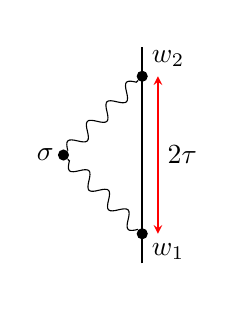
\begin{tikzpicture}[%
%scale=2,
>=stealth,
world/.style={inner sep=.5mm, fill=black, circle},
light/.style={decorate,decoration={coil, aspect=0}},
time/.style={thick},
tav/.style={<->, fill=red, draw=red},
rounded corners=0 mm,
anchor=base,
]

\node(pi1)  at (0,-0.5){};
\node(pi2)  at (0,2.5){};
\node[world](s)  at (-1,1){};
\node[world](w1) at (0,0){};
\node[world](w2) at (0,2){};
\draw[light](w1)--(s);
\draw[light](s)--(w2);
\draw[time](pi1)--(pi2);
\draw[tav](.2,0)--(.2,2) node[midway, right] {$2\tau$};

\node[anchor=east] at (s){$\sigma$};
\node[anchor=north west] at (w1){$w_1$};
\node[anchor=south west] at (w2){$w_2$};
\end{tikzpicture}
}

\felirat[anchor=north east]{1}{2}{1}{6.2}{0}{\footnotesize
\usetikzlibrary{decorations.pathmorphing}
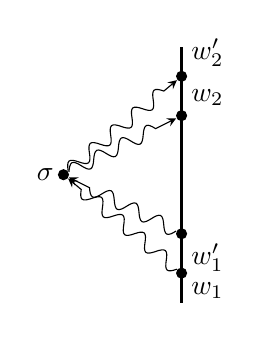
\begin{tikzpicture}[%
%scale=2,
>=stealth,
world/.style={inner sep=.5mm, fill=black, circle},
light/.style={->,decorate,decoration={coil, aspect=0}},
time/.style={thick},
tav/.style={<->, fill=red, draw=red},
rounded corners=0 mm,
anchor=base,
]

\node(pi1)  at (0,-0.5){};
\node(pi2)  at (0,3){};
\node[world](s)  at (-1.5,1.25){};
\node[world](w1) at (0,0){};
\node[world](w2) at (0,2){};
\node[world](w1') at (0,.5){};
\node[world](w2') at (0,2.5){};
\draw[light](w1)--(s);
\draw[light](s)--(w2);
\draw[light](w1')--(s);
\draw[light](s)--(w2');
\draw[time](pi1)--(pi2);
%\draw[tav](.2,0)--(.2,2) node[midway, right] {$2\tau$};

\node[anchor=east] at (s){$\sigma$};
\node[anchor=north west] at (w1){$w_1$};
\node[anchor=south west] at (w2){$w_2$};
\node[anchor=north west] at (w1'){$w_1'$};
\node[anchor=south west] at (w2'){$w_2'$};
\end{tikzpicture}
}
\end{frame}


\begin{frame}
\frametitle{Linearity}
\footnotesize

\begin{minipage}{7.75cm}
\magyi{Note that $a\parallel b$ does not imply $b\parallel a$. Imagine a normal clock $a$ and a clock $b$ which ticks exactly as fast as the normal on Mondays, but it ticks twice as fast as on every other day on the week. If $b$ is at rest to $a$ (from the outer point of view, in the model) then if $a$ starts signalling then she will say that $b$ is co-moving with her. But if $b$ will start signalling, then he will conclude that $a$ is more far away at Mondays than the usual. Note that even this strangeness is relative: in $b$'s perspective, $a$ is the strange, because her clock is ticking slower on Mondays; The only reason why $a$ thinks that $b$ is co-moving with her is that $a$ is closer to $b$ at Mondays, when its clock slows down. Now to rule out these situations, we introduce a definition which states that the clocks of $a$ and $b$ are not like the situation before: if $a$'s time evolves with a constant speed, $b$'s time must evolve with a constant speed as well.}
\end{minipage}


\dzsa{Definition} $\pi'$'s time is $\tau$-\emph{linear} according to $\pi$ iff
\[\mathrm{Lin}_{\tau}(\pi,\pi') \defekv \forall x,y,x',y' \left( \left(\begin{tomb}{c}\mathrm{ev}(\pi, x) \llfutureeq \mathrm{ev}(\pi',x') \\ \mathrm{ev}(\pi, y) \llfutureeq \mathrm{ev}(\pi',y')\end{tomb}\right) \lthen |x-y|=\tau\cdot |x'-y'|\right)
\]
$\mathrm{Lin}(\pi,\pi') \defekv \exists z \mathrm{Lin}_{z}(\pi,\pi')$

\dzsa{Proposition} $\forall a,b \big(\mathrm{Lin}(a,b)\lthen (a\parallel b \lthen b\parallel a)\big)$

\dzsa{proof} \magyi{$a\parallel b$ means that whenever $a$ bounces a photon to $b$, the elapsed time between the sending and receiving will be the same; let us call this elapsed time $2d$. Now by the linearity constraint, this means that arbitrary projections of such distance-measurement of $b$ will be some $z\cdot2d$, where $z$ is fixed. But these projections at the same time counts as distance-measurements of $a$ for $b$ as well (see the figure), so $b\parallel a$.}


\felirat[anchor=north east]{1}{2}{1}{6.2}{3}{\footnotesize
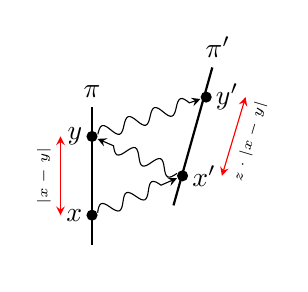
\begin{tikzpicture}[%
%scale=2,
>=stealth,
world/.style={inner sep=.5mm, fill=black, circle},
light/.style={->,decorate,decoration={coil, aspect=0}},
time/.style={thick},
tav/.style={<->, fill=red, draw=red},
geometria/.style={opacity=.3},
rounded corners=0 mm,
anchor=base,
]

\pgfmathsetmacro{\szelesseg}{1}
\pgfmathsetmacro{\magassag}{2}
\pgfmathsetmacro{\sebesseg}{0.3}
\pgfmathsetmacro{\leptek}{.5}

\node(pi)  at (0,-.5){};
\node(pi+)  at ([yshift=\magassag cm]pi){$\pi$};
\draw[time] (pi)--(pi+);

\node(pi')  at (\szelesseg,0){};
\node(pi'+)  at ([yshift=\magassag cm, xshift=\sebesseg*\magassag cm]pi'){$\pi'$};
\draw[time] (pi')--(pi'+);

\node[world](x) at (0,0){};
 \node[anchor=east] at (x) {$x$};
\node[world](x') at (\szelesseg+\leptek*\sebesseg,\leptek){};
 \node[anchor=west] at (x') {$x'$};

\node[world](y) at (0,2*\leptek){};
 \node[anchor=east] at (y) {$y$};
\node[world](y') at (\szelesseg+3*\leptek*\sebesseg,3*\leptek){};
 \node[anchor=west] at (y') {$y'$};
%\node[world](z) at (0,4*\leptek){};
% \node[anchor=east] at (z) {$z$};
%\node[world](z') at (\szelesseg+4*\leptek*\sebesseg,5*\leptek){};
 %\node[anchor=west] at (z') {$z'$};

\draw[light] (x)--(x');
\draw[light] (x')--(y);
\draw[light] (y)--(y');
%\draw[light] (y')--(z);
%\draw[light] (z)--(z');


\coordinate(xl)  at ([xshift=-.4cm]x);
\coordinate(yl)  at ([xshift=-.4cm]y);
\coordinate(x'l) at ([xshift= .5cm]x');
\coordinate(y'l) at ([xshift= .5cm]y');

\draw[tav] (xl)--(yl) node[midway, sloped, above]{\tiny $|x-y|$};
\draw[tav] (x'l)--(y'l) node[midway, sloped, below]{\tiny $z\cdot|x-y|$};

\end{tikzpicture}
}
\end{frame}

\begin{frame}
\frametitle{inertial synchronised co-movement}
\footnotesize

\begin{minipage}{8cm}
\magyi{Note that even $\mathrm{Lin}_1(\pi, \pi')\land \pi\parallel\pi'$ does not mean that they are synchronized:
\\ a) $\pi'$ can ticking backward compared to $\pi$,
\\ b) the same states are not necessarily simultaneous.% (to neither of them).
}

\bigskip

\dzsa{Definition} $\pi$ and $\pi'$ are \emph{inertial synchronised co-movers} iff $\pi'$ shows $x+\delta^i(\pi, \pi')$ whenever $\pi'$ sees that $\pi$ shows $x$.
\end{minipage}

\begin{multline*}
\pi\ISCM \pi' \defekv \forallin w {\Ex \pi}\forallin {w'} {\Ex \pi'} \big(w\llfutureeq w' \lthen \Pointsf (w',\pi')= \Pointsf (w,\pi)+\delta^i(\pi, \pi') \big)
\end{multline*}

\felirat[anchor=north east]{1}{2}{1}{6.2}{2.5}{\footnotesize
\usetikzlibrary{decorations.pathmorphing}
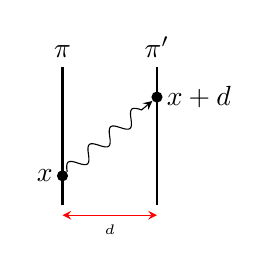
\begin{tikzpicture}[%
%scale=2,
>=stealth,
world/.style={inner sep=.5mm, fill=black, circle},
light/.style={->,decorate,decoration={coil, aspect=0}},
time/.style={thick},
tav/.style={<->, fill=red, draw=red},
geometria/.style={opacity=.3},
rounded corners=0 mm,
anchor=base,
]

\pgfmathsetmacro{\szelesseg}{1.2}
\pgfmathsetmacro{\magassag}{2}

\node(pi)  at (0,-.5){};
\node(pi+)  at ([yshift=\magassag cm]pi){$\pi$};
\draw[time] (pi)--(pi+);

\node(pi')  at (\szelesseg,-.5){};
\node(pi'+)  at ([yshift=\magassag cm]pi'){$\pi'$};
\draw[time] (pi')--(pi'+);

\node[world](x) at (0,0){};
 \node[anchor=east] at (x) {$x$};
\node[world](x') at (\szelesseg,1){};
 \node[anchor=west] at (x') {$x+d$};

\draw[light] (x)--(x');

\draw[tav] (0,-.5)--(\szelesseg,-.5) node[midway, below]{\tiny $d$};


\end{tikzpicture}
}
\end{frame}

\begin{frame}
\frametitle{Tarski's axioms of geometry}
\footnotesize

What we are going to do is to form a 3D geometry on the $\pi$-relative sets $\mathrm{Space}_\pi \defegy \{ a \in \mathbb C  : a\parallel \pi \}$ where $\pi\parallel \pi'\defekv \exists x \delta^i(\pi, \pi')=x$, i.e., on the set of clocks that are at rest compaired to $\pi$.

To do so, we need to express Tarski's primitive notions, betweenness $\Between(a,b,c)$ and equidistance $ab\EqDist cd$. This won't be hard since our basic toolkit (e.g. the theory of reals) is way more stronger than Tarski's.

\dzsa{Definition} We define betweenness using the triangle-(non)equality:
\[ \Between(\pi_1, \pi_2, \pi_3) \defekv \delta^i(\pi_1, \pi_2) + \delta^i(\pi_2, \pi_3) = \delta^i(\pi_1, \pi_3) \]
Recall that $\delta^i$ is a partial function, so betweenness implies the inertiality and co-movement of all of its arguments.

\bigskip

\dzsa{Definition} We define equidistance using the equality of distances:
\[ \pi_1\pi_2 \EqDist  \pi_3\pi_4 \defekv \delta^i(\pi_1, \pi_2) = \delta^i(\pi_3, \pi_4)\]

\bigskip

\dzsa{Definition} We define collinearity using betweenness:
\begin{multline*} \mathrm{Collinear}(\pi_1, \pi_2, \pi_3) \defekv \Between(\pi_1, \pi_2, \pi_3) \lor {}\\{}\lor \Between(\pi_3, \pi_1, \pi_2) \lor \Between(\pi_2, \pi_3, \pi_1)\end{multline*}

\end{frame}


\begin{frame}
\frametitle{Tarski's axioms}
\framesubtitle{}
\footnotesize

\begin{itemize}
\item $\forall ab \; ab\EqDist ba$ we have this by the symmetry of $\delta^i(a)$.
\end{itemize}
\end{frame}


\begin{frame}[t]
\frametitle{Coordinatization}
\framesubtitle{Basics of building coordinate systems: a 2D example}
\scriptsize
How can we give spatial coordinates on a 2D spacetime?
First we need someone to coordinatize, let this observer be $\pi$. Now we need another observer to determine a line (which covers the full space of a 2D spacetime), let this be $\pi_x$.
Now if we want to render spatial coordinates to the events occurring on that line, then we have to do the following:
Choose an origo for that line. Let this be $\pi$.
Choose a positive direction for that line. Let $\pi_x$ represent this positive direction.
The distance of any event for the origo is almost a perfect choice for a coordinate. The problem with this would be that distance can not be negative, while coordinates certainly can. To solve this, we introduce the following partial function based on betweenness:
\vspace{-1ex}
\[\mathrm{sign}_{\pi, \pi_x}(\pi') \defegy
\left\{\begin{tomb}{ll}
   1 & \textup{if } \Between(\pi, \pi', \pi_x) \lor \Between(\pi, \pi_x, \pi')
\\ -1 & \textup{if } \Between(\pi', \pi, \pi_x)
\end{tomb}\right.\]
\vspace{-1ex}
A more convenient definition is
\vspace{-1ex}
\begin{multline*}
\mathrm{sign}_{\pi, \pi_x}(\pi') =\tau\defekv
\Big(\big((\Between(\pi, \pi', \pi_x) \lor \Between(\pi, \pi_x, \pi')) \land \tau = 1 \big)\lor
\\ \big(\Between(\pi', \pi, \pi_x) \land \tau = -1\big)\Big)
\end{multline*}
Having such a function we can say (in 2D) that the spatial coordinate of an event $\sigma$ is $\mathrm{sign}_{\pi, \pi_x}(\pi_\sigma)\cdot \delta^i(\pi,\pi_\sigma)$, where $\pi_\sigma$ is some inertial clock that is parallel to $\pi$ and occurs in $\sigma$. Note that if that $\pi_\sigma$ is synchronized as well, then we have a good candidate for time coordinate as well: $\Pointsf (\sigma, \pi_\sigma)$.

\end{frame}


\begin{frame}[t]
\frametitle{Coordinatization}
\framesubtitle{Ortogonality and 4D coordinate systems}
\footnotesize
\begin{minipage}{8cm}
Every spatial line of an observer $\pi$ can be considered as a spacetime plane that is at rest w.r.t. $\pi$. Any such plane is determined by two inertial observer that is at rest w.r.t. $\pi$. Thus the ortogonality of lines of $\pi$ given by $\pi_1, \pi_2$ and $\pi'_1, \pi'_2$ would be a 4-place relation. But, to create coordinate systems, it is enough to speak about ortogonality of angles, i.e., ortogonality of lines going through $\pi_1$, $\pi_2$ and $\pi_1$ and $\pi_3$:

\dzsa{Idea} Lines $(\pi, \pi_1)$ and $(\pi,\pi_2)$ are orthogonal iff (see the figure on the right) $\pi\neq \pi_1$ and $\pi\neq \pi_2$ and the line  $(\pi,\pi_1)$ is the axis of symmetry of an isosceles triangle whose one leg is $(\pi_1, \pi_2)$, and the \emph{half of} the base is the segment $[\pi, \pi_2]$. Or in other words, there is a $w$ s.t. its distance from $\pi_1$ and $\pi$ is the same as the distance of $\pi_2$ from $\pi$, and $\pi_1$, and $\pi$ is between $\pi_2$ and $w$.
\end{minipage}
\vspace{-1ex}
\begin{multline*}
\mathrm{Ort}(\pi, \pi_1, \pi_2) \defekv \exists w (w \Ex \pi \land \lnot w \Ex \pi_3 )\land \exists w (w \Ex \pi \land \lnot w \Ex \pi_3 ) \land {}
\\ {}\land \exists w (\Between(\pi_2, \pi, w) \land \delta^i(\pi, \pi_2) = \delta^i(\pi, w) \land \delta^i(\pi_1, \pi_2)= \delta^i(\pi_1, w))
%\]%
\end{multline*}
\vspace{-2ex}
\[ \mathrm{CoordSys}(\pi, \pi_x, \pi_y, \pi_z)\defekv \mathrm{Ort}(\pi, \pi_x, \pi_y) \land \mathrm{Ort}(\pi, \pi_y, \pi_z)\land \mathrm{Ort}(\pi, \pi_x, \pi_z) \]



\felirat[anchor=north east]{1}{2}{1}{6.2}{2.75}{\footnotesize
\usetikzlibrary{decorations.pathmorphing}
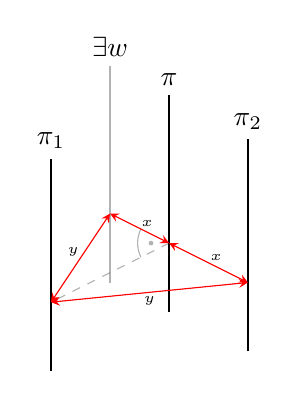
\begin{tikzpicture}[%
%scale=2,
>=stealth,
world/.style={inner sep=.5mm, fill=black, circle},
light/.style={->,decorate,decoration={coil, aspect=0}},
time/.style={thick},
tav/.style={<->, fill=red, draw=red},
geometria/.style={opacity=.3},
rounded corners=0 mm,
anchor=base,
]

\pgfmathsetmacro{\magassag}{3}
\pgfmathsetmacro{\vonalmagassag}{1}

\node(pi)  at (0,0){};
\node(pi+)  at ([yshift=\magassag cm]pi){$\pi$};
\draw[time] (pi)--(pi+);

\node(pi1)  at (-1.5,-0.75){};
\node(pi1+)  at ([yshift=\magassag cm]pi1){$\pi_1$};
\draw[time] (pi1)--(pi1+);

\node(pi2)  at (1,-0.5){};
\node(pi2+)  at ([yshift=\magassag cm]pi2){$\pi_2$};
\draw[time] (pi2)--(pi2+);

\node(w)  at (-.75,0.375){};
\node(w+)  at ([yshift=\magassag cm]w){$\exists w$};
\draw[time, geometria] (w)--(w+);

\coordinate (cpi) at ([yshift=\vonalmagassag cm]pi);
\coordinate (cpi1) at ([yshift=\vonalmagassag cm]pi1);
\coordinate (cpi2) at ([yshift=\vonalmagassag cm]pi2);
\coordinate (cw) at ([yshift=\vonalmagassag cm]w);

\draw[geometria, dashed] (cpi)--(cpi1);
\draw[tav] (cpi1)--(cpi2)node[midway, below, inner sep=0.5mm]{\tiny $y$};
\draw[tav] (cpi)--(cpi2)node[midway, above right, inner sep=0.2mm]{\tiny $x$};

\draw[tav] (cpi1)--(cw) node[midway, above left, inner sep=0.2mm]{\tiny $y$};
\draw[tav] (cpi)--(cw) node[midway, above right, inner sep=0.2mm]{\tiny $x$};

\clip (cpi)--(cpi1)--(cw)--cycle;
\draw[geometria] (cpi) circle (4mm);
\fill[geometria, fill=black] ([xshift=-2.3mm]cpi) circle (.3mm);

\end{tikzpicture}
}
\end{frame}


\begin{frame}[t]
\frametitle{Coordinatization}
\framesubtitle{Coordinate systems}
\footnotesize
$\mathrm{Coord}_{\pi, \pi_x, \pi_y, \pi_z}(\sigma) =  (\tau_t, \tau_x, \tau_y, \tau_z)\defekv $
\\[1ex]$\exists a_\sigma,a_x, a_y, a_z
\left(\begin{array}{l}
   \mathrm{CoordSys}(\pi, \pi_x, \pi_y, \pi_z)
\\ \sigma\Ex a_\sigma \land \mathrm{Sync}(\pi, a_\sigma)
%\\ \mathrm{Collinear}(\pi, \pi_x, a_x)
%\\ \mathrm{Collinear}(\pi, \pi_y, a_y)
%\\ \mathrm{Collinear}(\pi, \pi_z, a_z)
\\ \mathrm{Ort}(\pi, a_x, a_\sigma)
\\ \mathrm{Ort}(\pi, a_y, a_\sigma)
\\ \mathrm{Ort}(\pi, a_z, a_\sigma)
\\ \Points(\sigma, a_\sigma, \tau_t)
\\ \mathrm{sign}_{\pi, \pi_x}(a_x)\cdot \delta^i(a_x, a_\sigma)= \tau_x
\\ \mathrm{sign}_{\pi, \pi_y}(a_y)\cdot \delta^i(a_y, a_\sigma)= \tau_y
\\ \mathrm{sign}_{\pi, \pi_z}(a_z)\cdot \delta^i(a_z, a_\sigma)= \tau_z
\end{array}\right)$
\\[2ex]
\begin{minipage}{6cm}
Note that the last three equations -- by partiality of $\mathrm{sign}$ -- implies that $\mathrm{Collinear}(\pi, \pi_x, a_x)$, $\mathrm{Collinear}(\pi, \pi_y, a_y)$ and $\mathrm{Collinear}(\pi, \pi_z, a_z)$.
\end{minipage}

\felirat[anchor=north east]{1}{2}{1}{6.2}{2.2}{\footnotesize
\usetikzlibrary{decorations.pathmorphing}
\usetikzlibrary{intersections}
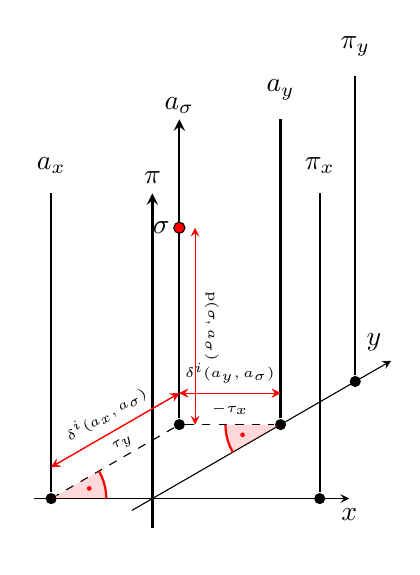
\begin{tikzpicture}[%
%scale=2,
>=stealth,
world/.style={inner sep=.5mm, fill=black, circle},
light/.style={->,decorate,decoration={coil, aspect=0}},
time/.style={thick},
tav/.style={<->, fill=red, draw=red},
geometria/.style={opacity=.3},
rounded corners=0 mm,
anchor=base,
]

\pgfmathsetmacro{\magassag}{4}
\pgfmathsetmacro{\yszog}{30}
\pgfmathsetmacro{\ytengelyhossz}{3.5}
\pgfmathsetmacro{\ytengelyhosszneg}{.3}
\pgfmathsetmacro{\xszog}{0}
\pgfmathsetmacro{\xtengelyhossz}{2.5}
\pgfmathsetmacro{\xtengelyhosszneg}{1.5}

\pgfmathsetmacro{\pix}{.85}
\pgfmathsetmacro{\piy}{.85}

\pgfmathsetmacro{\asszog}{70}
\pgfmathsetmacro{\astav}{1}
\pgfmathsetmacro{\asmag}{2.5}

\pgfmathsetmacro{\nyilmagassag}{.4}
\pgfmathsetmacro{\xvetirany}{\xszog}
\pgfmathsetmacro{\vetitovonalak}{2}

\coordinate(origo)  at (0,0);
\node(pi0)  at (0,-.5){};
\node(pi+)  at ([yshift=\magassag cm]origo){$\pi$};
\draw[time,->] (pi0)--(pi+);

\coordinate(x)  at ([shift=(\xszog:-\xtengelyhosszneg cm)]origo){};
\coordinate(x+) at ([shift=(\xszog:\xtengelyhossz cm)]origo);
\node[anchor=north] at (x+){$x$};
\draw[name path = xtengely, ->] (x)--(x+);

\coordinate(y)  at ([shift=(\yszog:-\ytengelyhosszneg cm)]origo){};
\coordinate(y+) at ([shift=(\yszog:\ytengelyhossz cm)]origo);
\node[anchor=south east] at (y+){$y$};
\draw[name path = ytengely, ->] (y)--(y+);

\node[world](as0) at ([shift=(\asszog:\astav cm)]origo){};
\node(as+) at ([shift=(90:\magassag cm)]as0){};
\node at (as+){$a_\sigma$};
\draw[time,->] (as0)--(as+);
\node[world, fill=red, draw=black](as) at ([shift=(90:\asmag cm)]as0){};
\node[anchor=east] at (as){$\sigma$};

\node[world](pix)  at ([shift=(\xszog:\pix*\xtengelyhossz cm)]origo){};
\node(pix+) at ([yshift=\magassag cm]pix){};
\draw[time] (pix)--(pix+);
\node[anchor=south] at (pix+){$\pi_x$};

\node[world](piy)  at ([shift=(\yszog:\piy*\ytengelyhossz cm)]origo){};
\node(piy+) at ([yshift=\magassag cm]piy){};
\draw[time] (piy)--(piy+);
\node[anchor=south] at (piy+){$\pi_y$};

\coordinate (as0xvet) at ([shift=(\xvetirany+\xszog: \vetitovonalak cm)]as0);
\path[name path = as0xvetline, opacity=.1] (as0)--(as0xvet);

\coordinate (as0yvet) at ([shift=(180+\yszog: \vetitovonalak cm)]as0);
\path[name path = as0yvetline, opacity=.1] (as0)--(as0yvet);

\node(ax0) [world, name intersections={of=as0yvetline and xtengely}]
at (intersection-1){};
\node(ax+) at ([yshift=\magassag cm]ax0){};
\node[anchor=south] at (ax+){$a_x$};
\draw[time] (ax0)--(ax+);

\draw[dashed] (as0)--(ax0);

\node(ay0) [world, name intersections={of=as0xvetline and ytengely}]
at (intersection-1){};
\node(ay+) at ([yshift=\magassag cm]ay0){};
\node[anchor=south] at (ay+){$a_y$};
\draw[time] (ay0)--(ay+);

\draw[dashed] (as0)--(ay0);

\coordinate(xcor1) at ([yshift=\nyilmagassag cm]ay0);
\coordinate(xcor2) at ([yshift=\nyilmagassag cm]as0);
\draw[tav] (xcor1)--(xcor2) node[midway, above]{\tiny $\delta^i(a_y, a_\sigma)$};
\draw[tav] (xcor1)--(xcor2) node[midway, below]{\tiny $-\tau_x$};

\coordinate(ycor1) at ([yshift=\nyilmagassag cm]ax0);
\coordinate(ycor2) at ([yshift=\nyilmagassag cm]as0);
\draw[tav] (ycor1)--(ycor2) node[midway, sloped, above]{\tiny $\delta^i(a_x, a_\sigma)$};
\draw[tav] (ycor1)--(ycor2) node[midway, sloped, below]{\tiny $\tau_y$};

\coordinate(tcor1) at ([xshift=.2cm]as0);
\coordinate(tcor2) at ([xshift=.2cm]as);

\draw[tav] (tcor2)--(tcor1) node[midway, sloped, above]{\tiny $\mathrm {p}(\sigma, a_\sigma )$};

\coordinate (clipax0) at (ax0);
\coordinate (clipay0) at (ay0);
\coordinate (clipas0) at (as0);
\clip (clipax0)--(origo)--(clipay0)--(clipas0);

\filldraw[red, thick, fill opacity=.15] (clipax0) circle (.7cm);
\fill[red] ([shift=(.5*\yszog:5mm)]ax0) circle (.3mm);

\filldraw[red, thick, fill opacity=.15] (clipay0) circle (.7cm);
\fill[red] ([shift=(180+.5*\yszog:5mm)]ay0) circle (.3mm);

\end{tikzpicture}
}
\end{frame}

\szakasz[Axiomatization of M]{Axiomatization of \\ Minkowski spacetimes}

%\begin{frame}[t]
%\frametitle{Guidelines}
%\footnotesize
%While choosing our axioms, we will follow the following criteria:
%\begin{itemize}
%\item The axioms should be formally simple. \\\magyi{The axioms should be so simple that they are presentable without abbreviations, using primitive predicates only.}
%\item The axioms should be conceptually simple. \\\magyi{The idea the axioms express should be easily imaginable.}
%\item The axioms should follow existing traditions.\\\magyi{Formulas that express well-known algebraic properties of certain relations or functions; formulas that are standard or reminding to standard axioms of traditional temporal logic or causal spaces; formulas that express basic operational ideas in the foundation of physics.}
%\item The axiomatization (as a didactic process in time) should follow the coordinatization process as close as the first three criteria permit it.
%\item If an axiom can be splitted into two or more different one without complicating it, then we will do so.
%\\ \magyi{Such an act usually helps the understanding of the logical structure of a theory because it permits more sophisticated differentiations between the models.}
%\end{itemize}
%\end{frame}

\begin{frame}[t]
\frametitle{Numbers}
\footnotesize
First we assume the FOL-theory of real numbers. Although this is a finitely axiomatizable theory, we omit to enlist all of its axioms.
\end{frame}

\begin{frame}[t]
\frametitle{Clocks}
\footnotesize
\begin{itemize}
\item $\forall a\forall x \exists w\;\Points(w,a,x)$
\\ \magyi{Clock states cover all numbers}
\item $\forall w \exists a \;w\Ex a$
\\ \magyi{There is no event without a clock}
\item $\forall {w,v}\forall a \big( \Pointsf(w,a) < \Pointsf (v,a) \liff w\future v\big)$
\\ \magyi{Clock are pointers evolving uniquely along causality.}
\item $\forall w,v \forall a \big(\Pointsf (w,a)=\Pointsf (v,a)\lthen w=v \big)$
\\ \magyi{Ticks determines the events}
%\item $\forall a,b \forall w\forall x \big((\Points (w,a,x)\liff \Points (v,a,x)) \lthen a=b\big)$
%\\ \magyi{Weak extensionality of clocks}
%\hfill \magyi{(The strong would be $(w\Ex a\liff v\Ex a) \lthen a=b$, see Shutz 1979}
\end{itemize}
\end{frame}

\begin{frame}[t]
\frametitle{Causality}
\footnotesize
\begin{itemize}
\item $\forall w,v,u \big((w\future v \land v \future u) \lthen w\future u\big)$
\\ \magyi{Causal future is transitive}
\item $\forall w,v\exists u (w\future u \land v \future u)$
\\ \magyi{Causal future is directed}
\item $\forall w,v\exists u (w\past u \land v \past u)$
\\ \magyi{Causal past is directed}
\end{itemize}
\end{frame}



\begin{frame}[t]
\frametitle{Coordinatization}
\footnotesize
\begin{itemize}
\item $\forall a \forall w \existsin {v_1, v_2}{\Ex a} \;v_1\llfutureeq w\llfutureeq v_2$
\\ \magyi{Every event is accessible to all clocks (AxEv)}
\item $\forall a \existsin {w_1, w_2}{\Ex a} \forall w \;\big((w_1\llfutureeq v \land w_2\llfutureeq v) \lthen w_1=w_2\big)$
\\ \magyi{No light signal can catch up with a light signal that was sent before from the same clock.}
\item $\forall a \existsin {w_1, w_2}{\Ex a} \forall w \;\big((v\llfutureeq w_1 \land v\llfutureeq w_2) \lthen w_1=w_2\big)$
\\ \magyi{No light signal can lag behind a light signal that arrived to the same event (of a clock).}
\item $\forall a \forall w \exists b (w\Ex b \land \mathrm{Sync}(a,b))$
\\ \magyi{For every clock and for every event there is a synchronized co-moving clock passing through that event.}
\item $\forall w_1 \forall w_2\forall w_3 \exists w',w_2' \big(w_1\llfuture w_2\llfuture w_3\land \lnot w_1\llfuture w_3) \lthen \exists w_2'(w_2\neq w_2' w_1\llfuture w_2\llfuture w_3) \big)$
\\ \magyi{For every clock and for every event there is a synchronized co-moving clock passing through that event.}
\item $(\delta^i(a, b)=x \land \mathrm{ev}(a,-x)\future \mathrm{ev}(b,0) )\lthen \forall y (\mathrm{ev}(a,y-x)\future \mathrm{ev}(b,y)) $
\\ \magyi{Every co-moving clock uses the same measure system}
\end{itemize}
\end{frame}


\end{document} 